\documentclass[11pt]{article}
\usepackage[margin=1in]{geometry}
\usepackage{graphicx,amsmath,amssymb,booktabs,hyperref,xcolor,subcaption,listings}
\usepackage[font=small]{caption}
\usepackage{parskip}          % blank line between paragraphs, no indent
\usepackage{titlesec}
\titlespacing*{\paragraph}{0pt}{1.2ex plus .5ex}{0.8em}
\definecolor{codebg}{gray}{0.96}
\lstset{language=Python,basicstyle=\ttfamily\footnotesize,breaklines=true,frame=single,
  rulecolor=\color{gray!60},backgroundcolor=\color{codebg},columns=fullflexible,
  keywordstyle=\color{blue!70!black}\bfseries,commentstyle=\color{green!45!black}\itshape,
  stringstyle=\color{red!60!black},aboveskip=0.6em,belowskip=0.6em,linewidth=\linewidth}
% code block that never splits across pages
\lstnewenvironment{codeblock}{\endgraf\nopagebreak[4]\noindent\minipage{\linewidth}}{\endminipage\endgraf}
\newcommand{\todo}[1]{\textcolor{red}{[TODO: #1]}}
\newcommand{\FIDddpmunet}{\textbf{8.3}}
\newcommand{\FIDddpmvit}{10.5}
\newcommand{\FIDfmunet}{11.6}
\newcommand{\FIDfmvit}{11.7}
\newcommand{\MNISTFIDsentence}{ The FID scores in Table~\ref{tab:mnist} agree: DDPM with the U-Net is
the best model (8.3), and DDPM scores better than FM for both backbones (8.3 vs.\ 11.6 for the U-Net,
10.5 vs.\ 11.7 for the ViT).}
\newcommand{\MNISTtimesentence}{ In practice, generating the 1{,}000 FID images (plus computing FID) on
a laptop GPU took about 3 minutes for FM with the ViT but about 73 minutes for DDPM with the ViT. DDPM's
better FID therefore comes at roughly $20\times$ the sampling time.}


\title{CS 771 Fall 2026 --- Homework Assignment 3}
\author{Karthik Reddy Jannupalli \and Sanjana Kallingal \and Penchala Siva Prasanth Kasa}
\date{November 2026}

\begin{document}
\maketitle

\section*{Team contributions}
All three members contributed equally.
\begin{itemize}
\item \textbf{Karthik Reddy Jannupalli:} implemented the U-Net decoder and the ViT (LightningDiT)
forward pass; wrote the prediction-networks section and the U-Net vs.\ ViT comparison.
\item \textbf{Sanjana Kallingal:} implemented DDPM and flow matching (losses and sampling); set up the
cloud GPU and ran the MNIST experiments; wrote the DDPM, flow matching and MNIST results sections.
\item \textbf{Penchala Siva Prasanth Kasa:} implemented latent modeling with TAESD in DDPM and FM;
ran the MiniImageNet experiments and FID evaluation; wrote the latent modeling and MiniImageNet sections.
\end{itemize}
All members tested the code, reviewed the results and edited the final report together.

\section{Setup}
We implemented DDPM and flow matching (rectified flow), the U-Net decoder, the ViT (LightningDiT)
forward pass, and latent-space modeling with the pretrained TAESD autoencoder. All six required
experiments were trained on a Google Cloud \texttt{n1-standard-4} instance with one NVIDIA Tesla T4 (16\,GB).

We used the supplied configurations unchanged except for one line, \texttt{dtype: "fp16"}, which
turns on the mixed-precision training already supported by \texttt{train.py}. This uses the T4's
tensor cores and made training about $1.6\times$ faster; model, optimizer, epoch and sampling
settings are all the supplied defaults. To save time we ran two experiments at once on the same GPU,
so the reported training times are for a shared GPU (they are still comparable between runs).
No packages beyond \texttt{requirements.txt} are needed. Classifier-free guidance (bonus) was not
implemented, so all samples are generated with plain class conditioning.

\textbf{MNIST:} $1\times28\times28$ images in $[-1,1]$, batch size 64, learning rate $10^{-4}$,
30 epochs (28{,}140 iterations).
\textbf{MiniImageNet:} $3\times128\times128$ images encoded to $4\times16\times16$ latents, batch
size 64, learning rate $2\times10^{-4}$, 80 epochs (62{,}500 iterations). All sample grids and FID
scores use the EMA (exponential moving average) weights.

\section{Prediction networks}
Both backbones implement a function $f_\theta(x, c, t)$ of the noisy input $x$, the class label $c$
and the time $t$. DDPM uses it to predict noise, and FM uses it to predict velocity. In both
networks, $t$ is converted to a vector by a sinusoidal encoding followed by a small MLP, and $c$ is
mapped to a learned embedding vector. (During training the label is replaced by a ``null'' class 10\%
of the time, which would allow CFG later.)

\subsection{U-Net decoder}
\begin{codeblock}
for resblock, transformer, upsample in self.decoder:
    x = torch.cat([x, encoder_output.pop()], dim=1)   # skip connection
    x = resblock(x, t)                                # uses time
    if transformer:
        x = transformer(x, c)                         # uses class
    if upsample:
        x = upsample(x)
\end{codeblock}
\paragraph{Implementation.} The decoder mirrors the encoder. While encoding, every block saved its output
in the list \texttt{encoder\_output}. Each decoder block takes the most recently saved output
(\texttt{pop()} returns them in reverse order, so the spatial sizes match) and concatenates it with
the current features along the channel dimension. These \emph{skip connections} let fine spatial
detail from the encoder bypass the low-resolution bottleneck. The combined features then pass through
a residual block, a spatial transformer (only at the levels that use attention), and an upsampling
layer (except at the last level). The existing output layer maps the result back to the image or
latent channels.

\paragraph{How time and class are used.} \emph{Time} is used in every residual block: the time
embedding is projected to the block's number of channels and added to the feature map after the first
convolution, as a per-channel shift. This tells each layer how noisy its input is. \emph{Class} is
used in the spatial transformer blocks (encoder, middle and decoder). After self-attention over the
pixels, a \emph{cross-attention} layer uses the image features as queries and the class embedding as
keys and values, so every location in the image can read the class information.

\subsection{ViT (LightningDiT) forward pass}
\begin{codeblock}
c = t + y                      # one conditioning vector per image
for block in self.blocks:
    x = block(x, c)            # transformer blocks with adaLN-Zero
x = self.final_layer(x, c)     # map each token back to its 2x2 patch
x = self.unpatchify(x)         # reassemble patches into (N, C, H, W)
\end{codeblock}
\paragraph{Implementation.} The supplied code splits the input into $2\times2$ patches, embeds each patch
as a token, adds positional embeddings, and computes the time embedding $t$ and class embedding $y$.
Following DiT, we add them into a single conditioning vector $c=t+y$, run the tokens through all
transformer blocks, apply the final layer, and reassemble the patches into an output with the same
shape as the input.

\paragraph{How time and class are used.} Unlike the U-Net, the ViT does not attend to the label. Instead,
$c$ controls \emph{adaptive layer normalization (adaLN-Zero)}. In each block a small MLP maps $c$ to
per-channel shift, scale and gate values; these modulate the normalized tokens before the attention
and MLP layers and scale (gate) their residual outputs. The final layer is modulated the same way.
The gates are initialized to zero, so each block starts as the identity function and gradually learns
how strongly time and class should change the features. Time and class therefore affect every token
globally, through feature modulation rather than attention.

\section{DDPM}
\paragraph{Loss (Algorithm 1).}\mbox{}
\begin{codeblock}
noise = torch.randn_like(x_start)                               # eps ~ N(0, I)
t = torch.randint(0, self.timesteps, (batch_size,), device=...) # t ~ U{0..T-1}
x_t = self.q_sample(x_start, t, noise=noise)                    # noisy image
loss = F.mse_loss(self.model(x_t, label, t), noise)
\end{codeblock}
For each training image we pick a random timestep $t$ and random Gaussian noise $\epsilon$, and jump
directly to the noisy image $x_t=\sqrt{\bar\alpha_t}\,x_0+\sqrt{1-\bar\alpha_t}\,\epsilon$ using the
supplied \texttt{q\_sample}. The network is trained to predict the noise that was added, with the
simplified loss $\|\epsilon-\epsilon_\theta(x_t,c,t)\|^2$.

\paragraph{One reverse step (Equation 11).}\mbox{}
\begin{codeblock}
pred_noise = self.model(x, label, t)
mean = sqrt_recip_alphas_t * (x - betas_t / sqrt_one_minus_alphas_cumprod_t * pred_noise)
if t_index == 0:
    return mean
return mean + torch.sqrt(posterior_variance_t) * torch.randn_like(x)
\end{codeblock}
Given $x_t$, the network's noise prediction gives the mean of the less-noisy image,
$\mu_\theta=\frac{1}{\sqrt{\alpha_t}}\big(x_t-\frac{\beta_t}{\sqrt{1-\bar\alpha_t}}\epsilon_\theta(x_t,c,t)\big)$.
We then add a small amount of fresh noise with variance $\sigma_t^2$ (the supplied posterior variance).
At the last step ($t=0$) we return the mean without adding noise.

\paragraph{Sampling (Algorithm 2).} \texttt{generate} starts from pure noise $x_T\sim\mathcal N(0,I)$ and
applies the reverse step for $t=T-1,\dots,0$ ($T=500$), using the requested labels at every step.
The result is clamped to $[-1,1]$ and mapped to $[0,1]$ by the supplied post-processing.

\section{Flow matching (rectified flow)}
\paragraph{Loss.}\mbox{}
\begin{codeblock}
noise = torch.randn_like(x_start)                       # z ~ N(0, I)
t = torch.rand(batch_size, device=...)                  # t ~ U[0, 1]
t_ = t.view(batch_size, 1, 1, 1)
x_t = (1 - t_) * noise + t_ * x_start                   # point on the path
loss = F.mse_loss(self.model(x_t, label, t), x_start - noise)
\end{codeblock}
\begin{itemize}
\item \textbf{Training path:} the straight line between a noise sample $z$ and a real image $x$,
$x_t=(1-t)z+tx$, which is pure noise at $t=0$ and the clean image at $t=1$ (Eq.~1).
\item \textbf{Prediction target:} the velocity along that line, $dx_t/dt=x-z$ (Eq.~2). It is the same
at every point of a given line, and the network learns it with a mean-squared error (Eq.~3).
\item \textbf{Time distribution:} $t$ is sampled uniformly in $[0,1]$, so every part of the path gets
equal training weight. It is the simplest choice and needs no tuning. Time is passed to the network
as a real number in $[0,1]$.
\end{itemize}

\paragraph{Sampling.}\mbox{}
\begin{codeblock}
for i in range(self.timesteps):                          # T = 10
    t = torch.full((batch_size,), i * self.dt, device=...)  # dt = 1 / T
    imgs = imgs + self.dt * self.model(imgs, labels, t)
\end{codeblock}
We start from noise at $t=0$ and follow the predicted velocity to $t=1$ using the forward Euler method
(Eq.~5): at each of the $T=10$ steps we move by $\Delta t\,f_\theta(y,c,t)$ with $\Delta t=1/T$.
Unlike DDPM, no noise is added after the starting point, so sampling is deterministic.

\section{MNIST results}
\begin{figure}[!htbp]
\centering
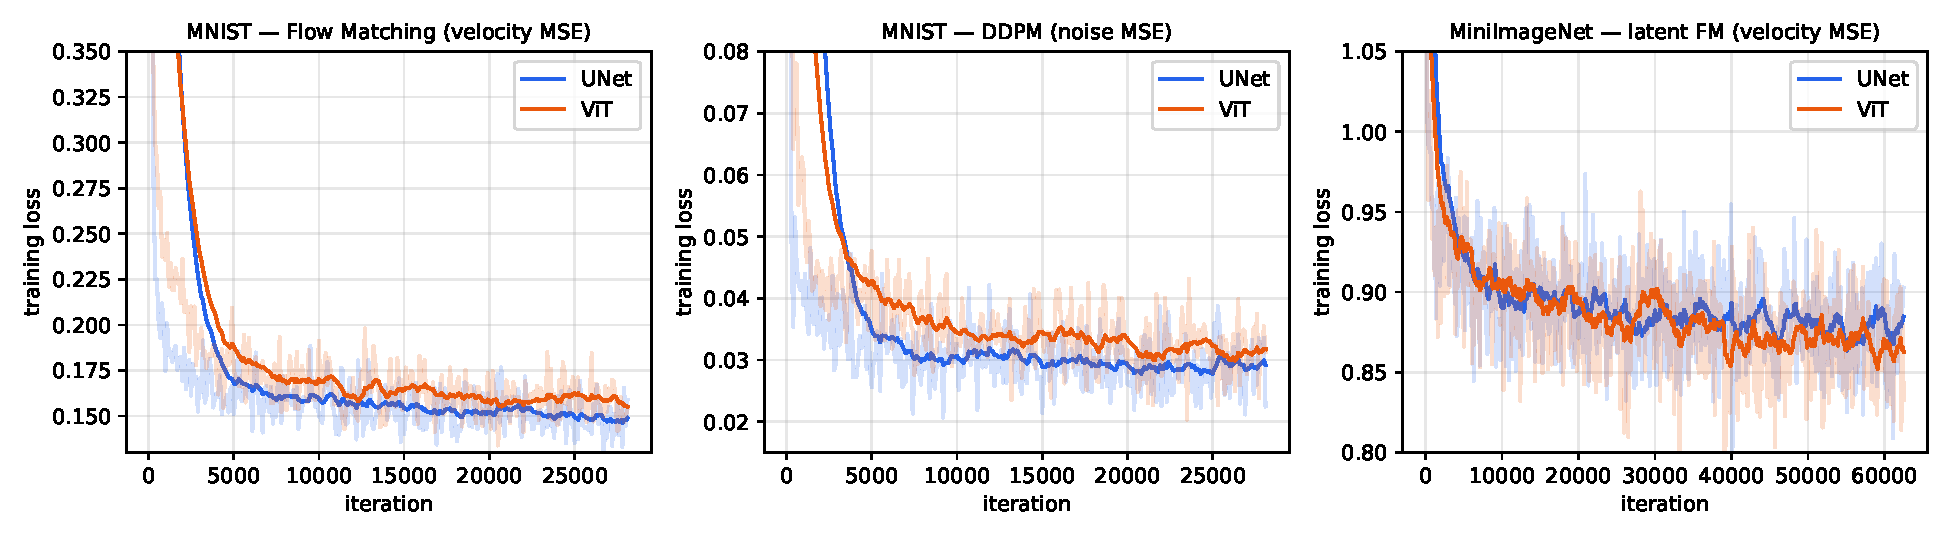
\includegraphics[width=\linewidth]{figs/curves.pdf}
\caption{Training loss (light: raw values every 100 iterations; dark: smoothed). Left and middle: MNIST
FM and DDPM. Right: MiniImageNet latent FM. FM and DDPM losses measure different targets (velocity vs.\
noise), so their values cannot be compared with each other.}
\label{fig:curves}
\end{figure}

\begin{figure}[!htbp]
\centering
\begin{subfigure}{0.24\linewidth}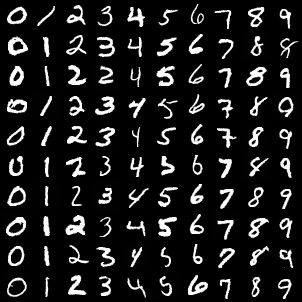
\includegraphics[width=\linewidth]{figs/mnist_ddpm_unet.png}\caption{DDPM, U-Net}\end{subfigure}
\begin{subfigure}{0.24\linewidth}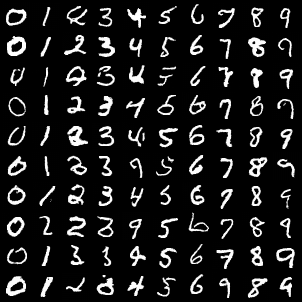
\includegraphics[width=\linewidth]{figs/mnist_ddpm_vit.png}\caption{DDPM, ViT}\end{subfigure}
\begin{subfigure}{0.24\linewidth}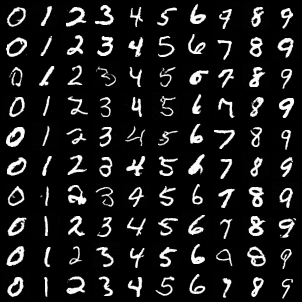
\includegraphics[width=\linewidth]{figs/mnist_fm_unet.png}\caption{FM, U-Net}\end{subfigure}
\begin{subfigure}{0.24\linewidth}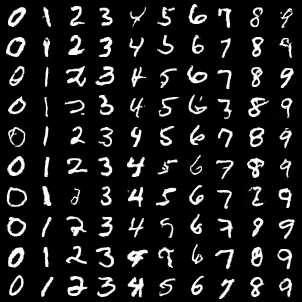
\includegraphics[width=\linewidth]{figs/mnist_fm_vit.png}\caption{FM, ViT}\end{subfigure}
\caption{MNIST samples after the final epoch (EMA model). Column $k$ is conditioned on digit $k$, and
each row uses different starting noise.}
\label{fig:mnist}
\end{figure}

\begin{table}[!htbp]
\centering
\begin{tabular}{llrrrrr}
\toprule
Method & Backbone & Params & Sampling steps & Train time & s/iter & FID$^*$ \\
\midrule
DDPM & U-Net & 7.46M & 500 & 2h58m & 0.38 & \FIDddpmunet \\
DDPM & ViT   & 5.54M & 500 & 2h59m & 0.38 & \FIDddpmvit \\
FM   & U-Net & 7.46M & 10  & 2h56m & 0.38 & \FIDfmunet \\
FM   & ViT   & 5.54M & 10  & 2h43m & 0.35 & \FIDfmvit \\
\bottomrule
\end{tabular}
\caption{MNIST summary (30 epochs, shared T4). $^*$Not required; FID from 1{,}000 generated images
(100 per class) against the MNIST test split, using \texttt{eval.py}.}
\label{tab:mnist}
\end{table}

\paragraph{Training curves.} All four runs train smoothly (Fig.~\ref{fig:curves}). Most of the
improvement happens in the first $\sim$5{,}000 iterations, followed by a slow decrease. For both
methods the U-Net ends with a slightly lower loss than the ViT (FM: about 0.15 vs.\ 0.16; DDPM: about
0.029 vs.\ 0.032). The ViT also starts more slowly, which is expected because its adaLN gates start at zero.

\paragraph{Generation quality.} All four models produce recognizable digits, and most cells in
Fig.~\ref{fig:mnist} show the requested digit, with natural variety in thickness, slant and style. The
U-Net models are the cleanest. DDPM with the U-Net gives smooth strokes with almost no failures, and FM
with the U-Net is close behind, with a few wobbly or broken strokes. The ViT models make noticeably more
mistakes with both methods, such as malformed digits or digits that look like another class (e.g., 4s
resembling 9s, or 3s and 5s that are hard to tell apart). This matches their higher training loss.\MNISTFIDsentence

\paragraph{U-Net vs.\ ViT.} The U-Net has more parameters (7.5M vs.\ 5.5M) and took about the same time
per iteration. Its convolutions have a built-in preference for local patterns, which suits small
images and helps it learn faster. The ViT treats the image as $14\times14=196$ patch tokens and must
learn spatial structure from data, so with only 30 epochs it is slightly behind.

\paragraph{FM vs.\ DDPM, and sampling cost.} Training costs the same for both methods: one network
call per training image. Sampling is very different: DDPM needs 500 network calls per image, while FM
needs only 10, which is $50\times$ fewer. Even so, FM's quality is close to DDPM's. This works because
rectified flow learns nearly straight paths from noise to image, which a few large Euler steps can
follow, while DDPM's reverse process is trained to take many small, noisy steps.\MNISTtimesentence

\section{Latent modeling and MiniImageNet}
\paragraph{Implementation.} With \texttt{use\_vae}, the data loader returns images in $[0,1]$, and the
model constructor already loads the frozen TAESD and sets the working shape to the latent shape
($4\times16\times16$ for $128\times128$ images). We added the same two steps to both DDPM and FM:
\begin{codeblock}
# compute_loss: turn images into latents first (frozen encoder, no gradients)
if self.use_vae:
    with torch.no_grad():
        x_start = self.vae.encode(x_start)
# ... the loss is then computed on latents exactly as in pixel space ...

# generate: after the sampling loop, decode latents back to images in [0, 1]
if self.use_vae:
    imgs = self.vae.decode(imgs)
\end{codeblock}
Everything else stays the same; the noise simply has the latent shape. We checked that TAESD latents of
MiniImageNet images have a standard deviation of about 0.95, already close to the unit variance of the
noise, so no extra scaling factor was needed. We also checked that no gradients reach the autoencoder.
The decoder already outputs images in $[0,1]$, so post-processing only clamps the values.

\paragraph{How latent modeling differs from pixel space.} In pixel space the model must generate every
one of the $3\times128\times128=49{,}152$ values, including fine details that matter little to how the
image looks. In latent space it generates $4\times16\times16=1{,}024$ values, $48\times$ fewer, that
mostly describe the overall content and layout; the pretrained decoder fills in textures and fine
detail. Each network call is therefore much cheaper (the ViT handles 64 tokens instead of 4{,}096), which
is what makes training on $128\times128$ images feasible on a single T4. The trade-off is that the
decoder's quality limits the best possible images, and errors are measured in latent space rather than
on the pixels.

\begin{figure}[!htbp]
\centering
\begin{subfigure}{0.49\linewidth}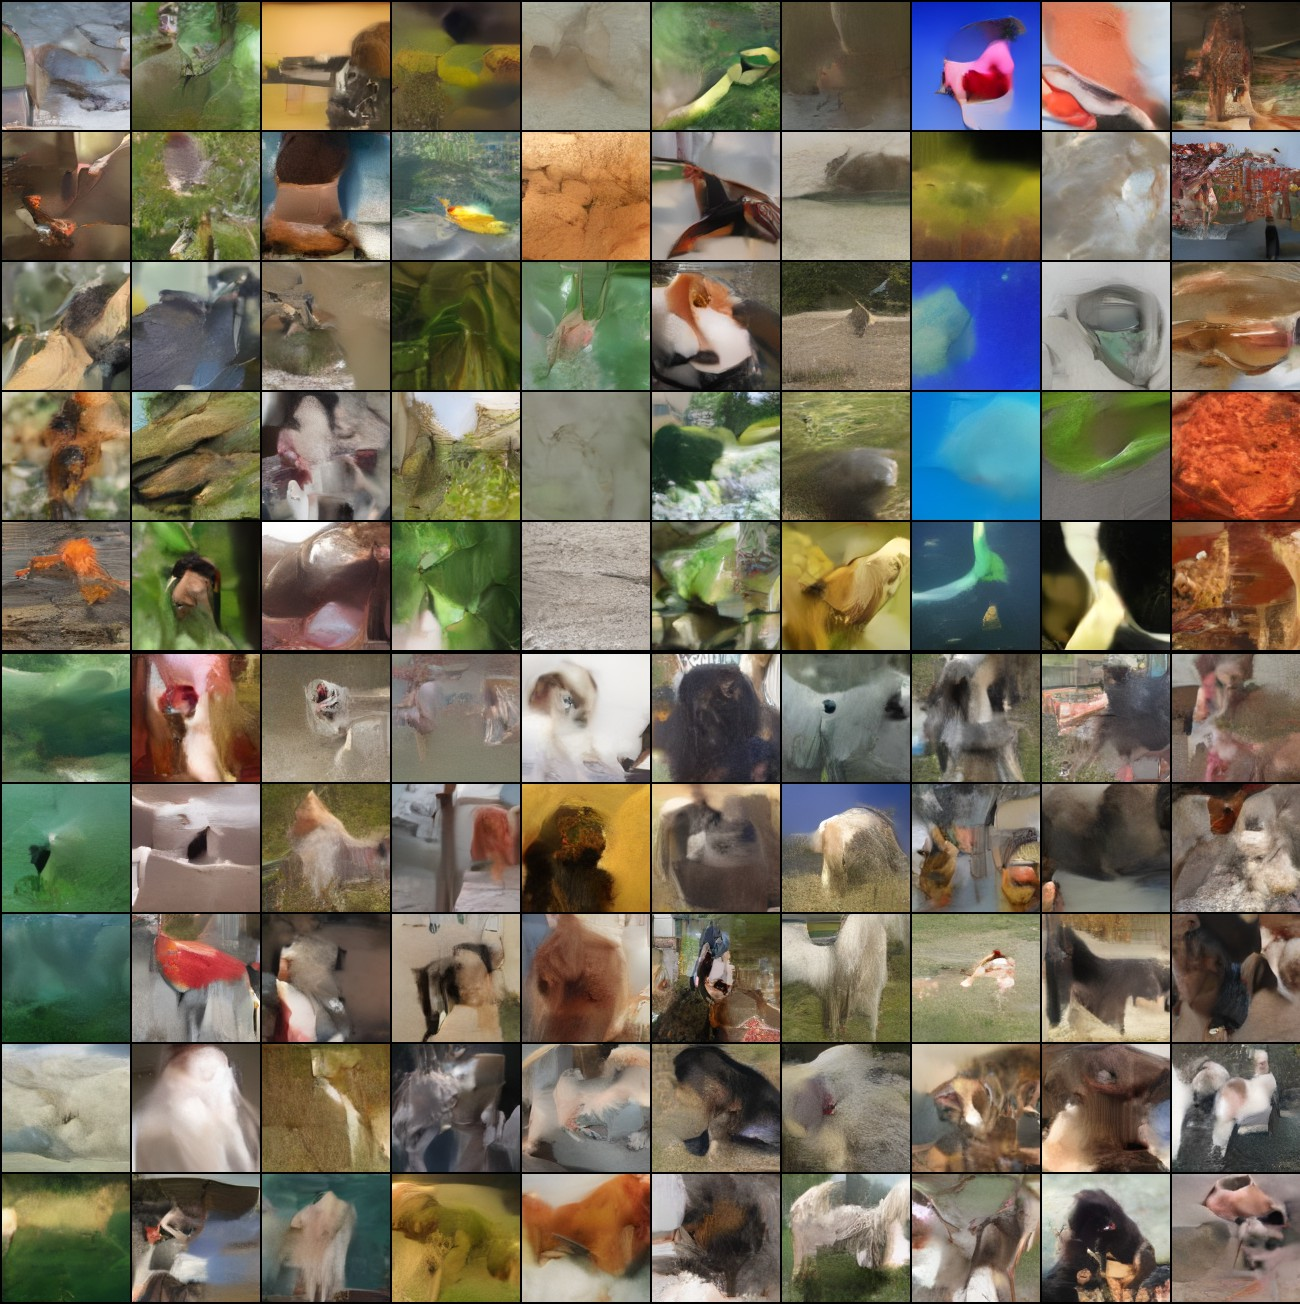
\includegraphics[width=\linewidth]{figs/mini_unet_ep79.jpg}\caption{U-Net}\end{subfigure}\hfill
\begin{subfigure}{0.49\linewidth}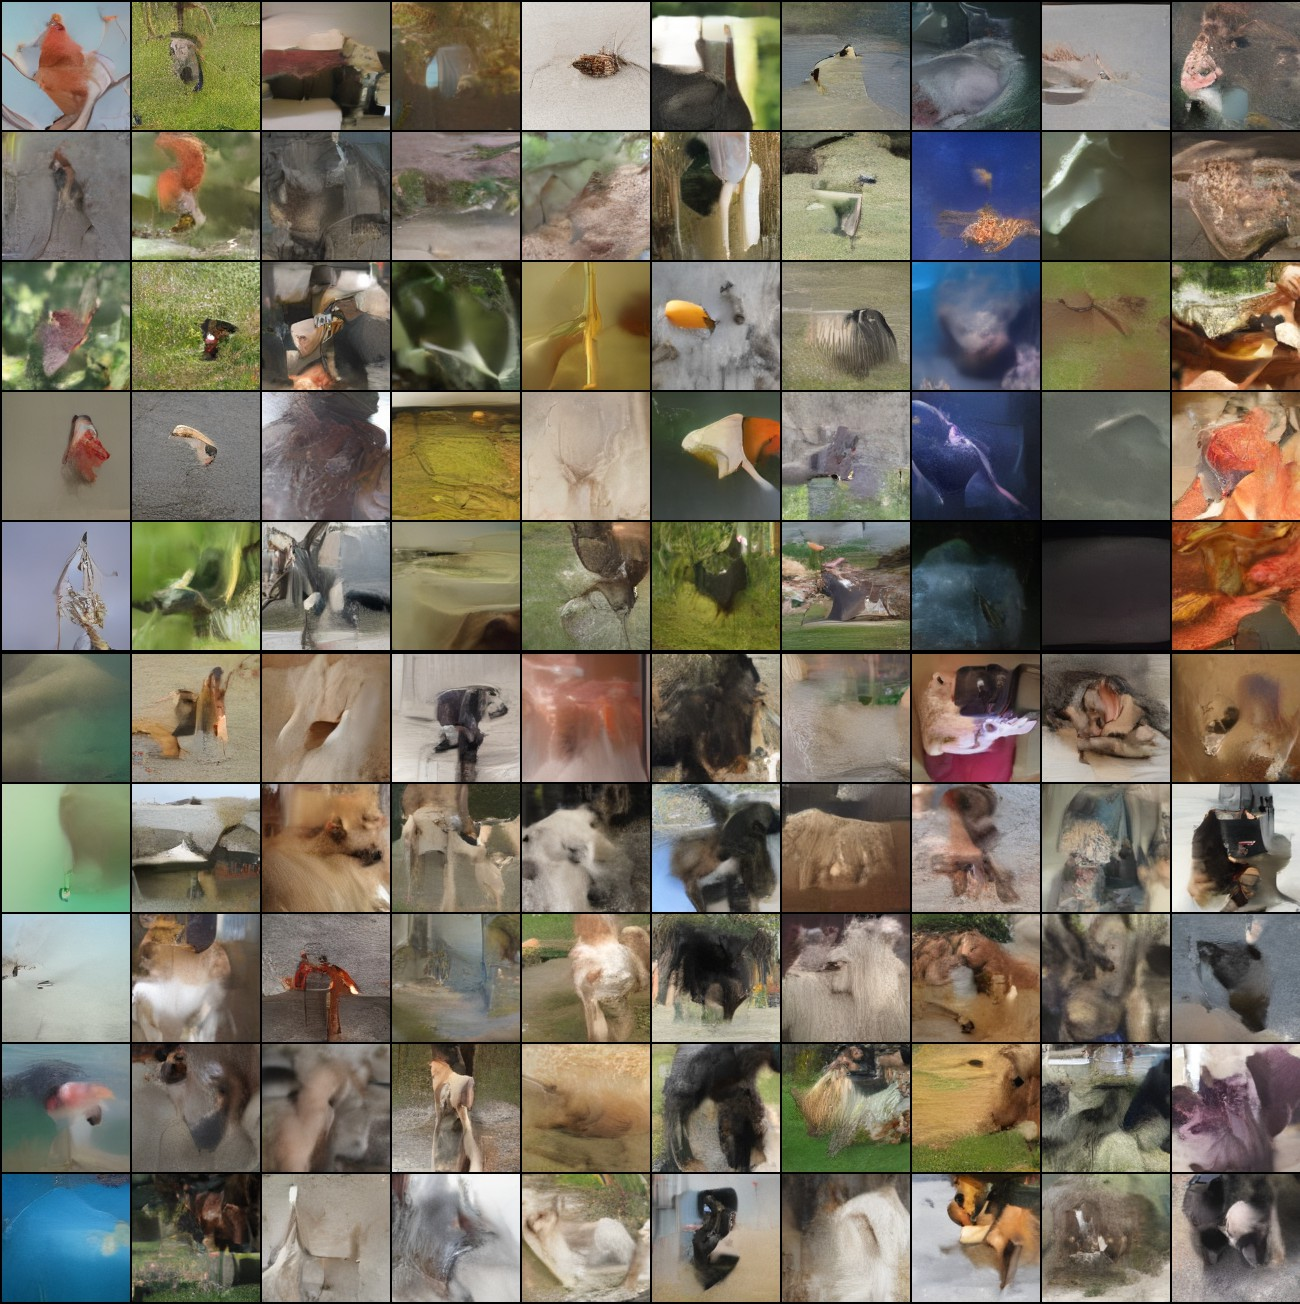
\includegraphics[width=\linewidth]{figs/mini_vit_ep79.jpg}\caption{ViT}\end{subfigure}
\caption{Final MiniImageNet samples (EMA, 10 Euler steps) for classes 0--9 (top five rows) and 10--19
(bottom five rows). Each column is one class with five different samples. The full 100-class grids
are in \texttt{results/}.}
\label{fig:mini}
\end{figure}

\begin{figure}[!htbp]
\centering
\begin{subfigure}{0.32\linewidth}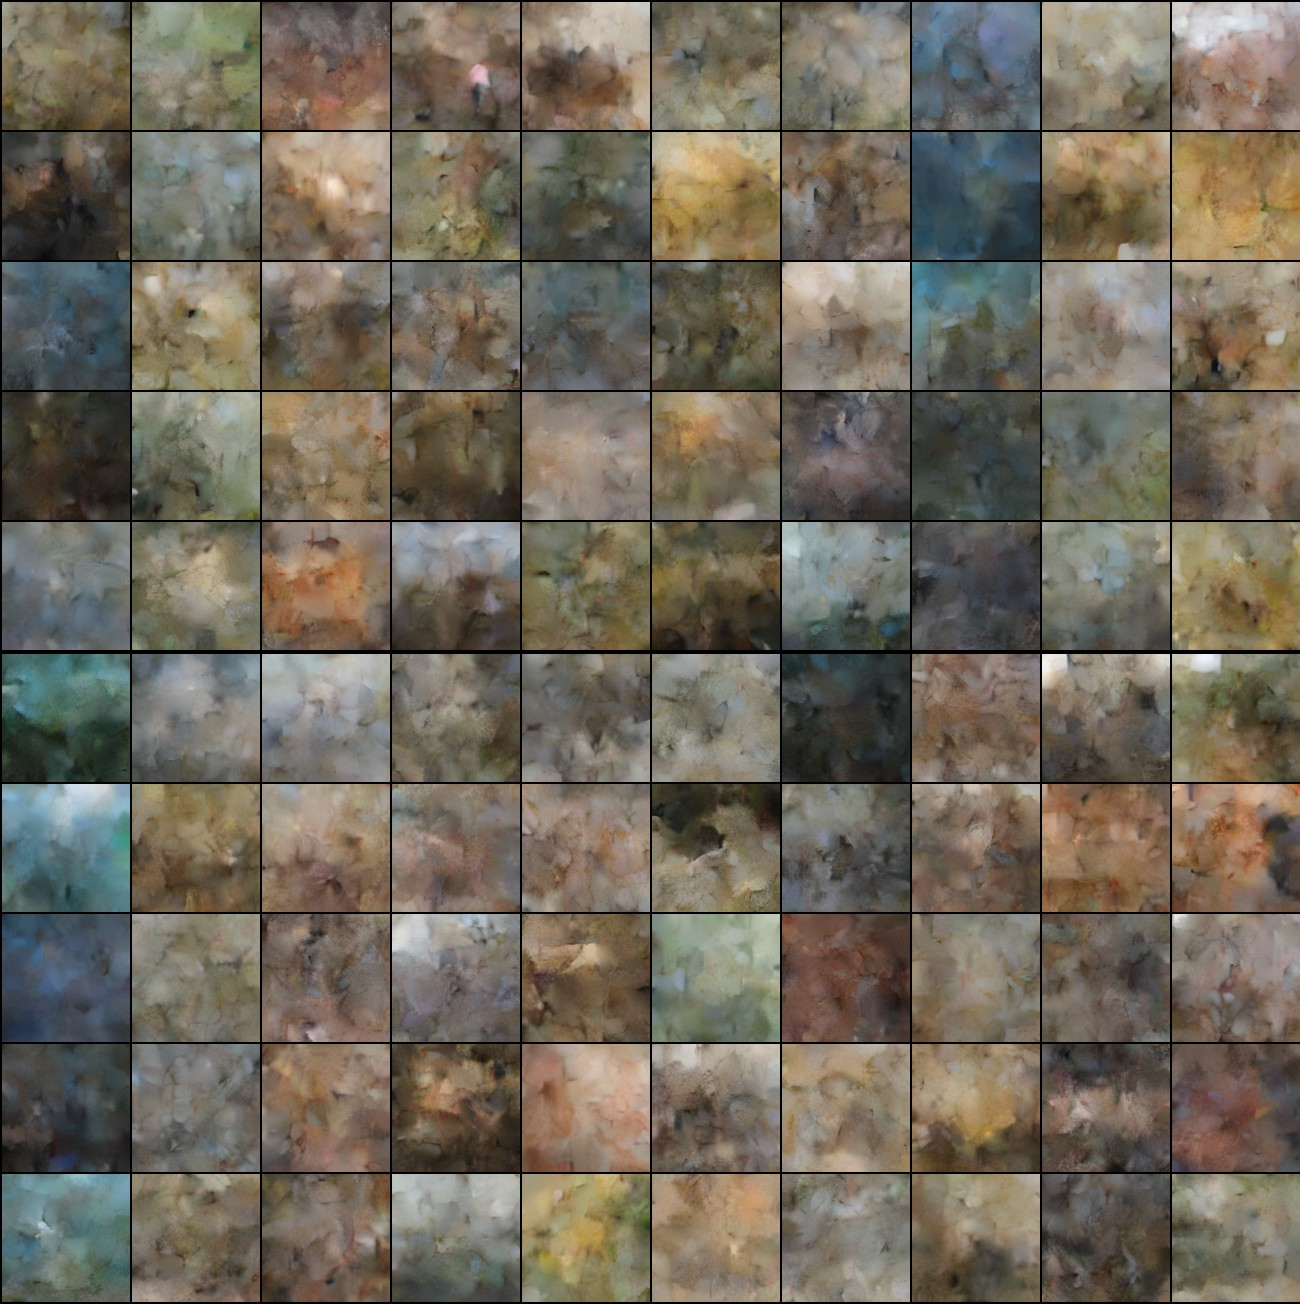
\includegraphics[width=\linewidth]{figs/mini_vit_ep4.jpg}\caption{epoch 5}\end{subfigure}
\begin{subfigure}{0.32\linewidth}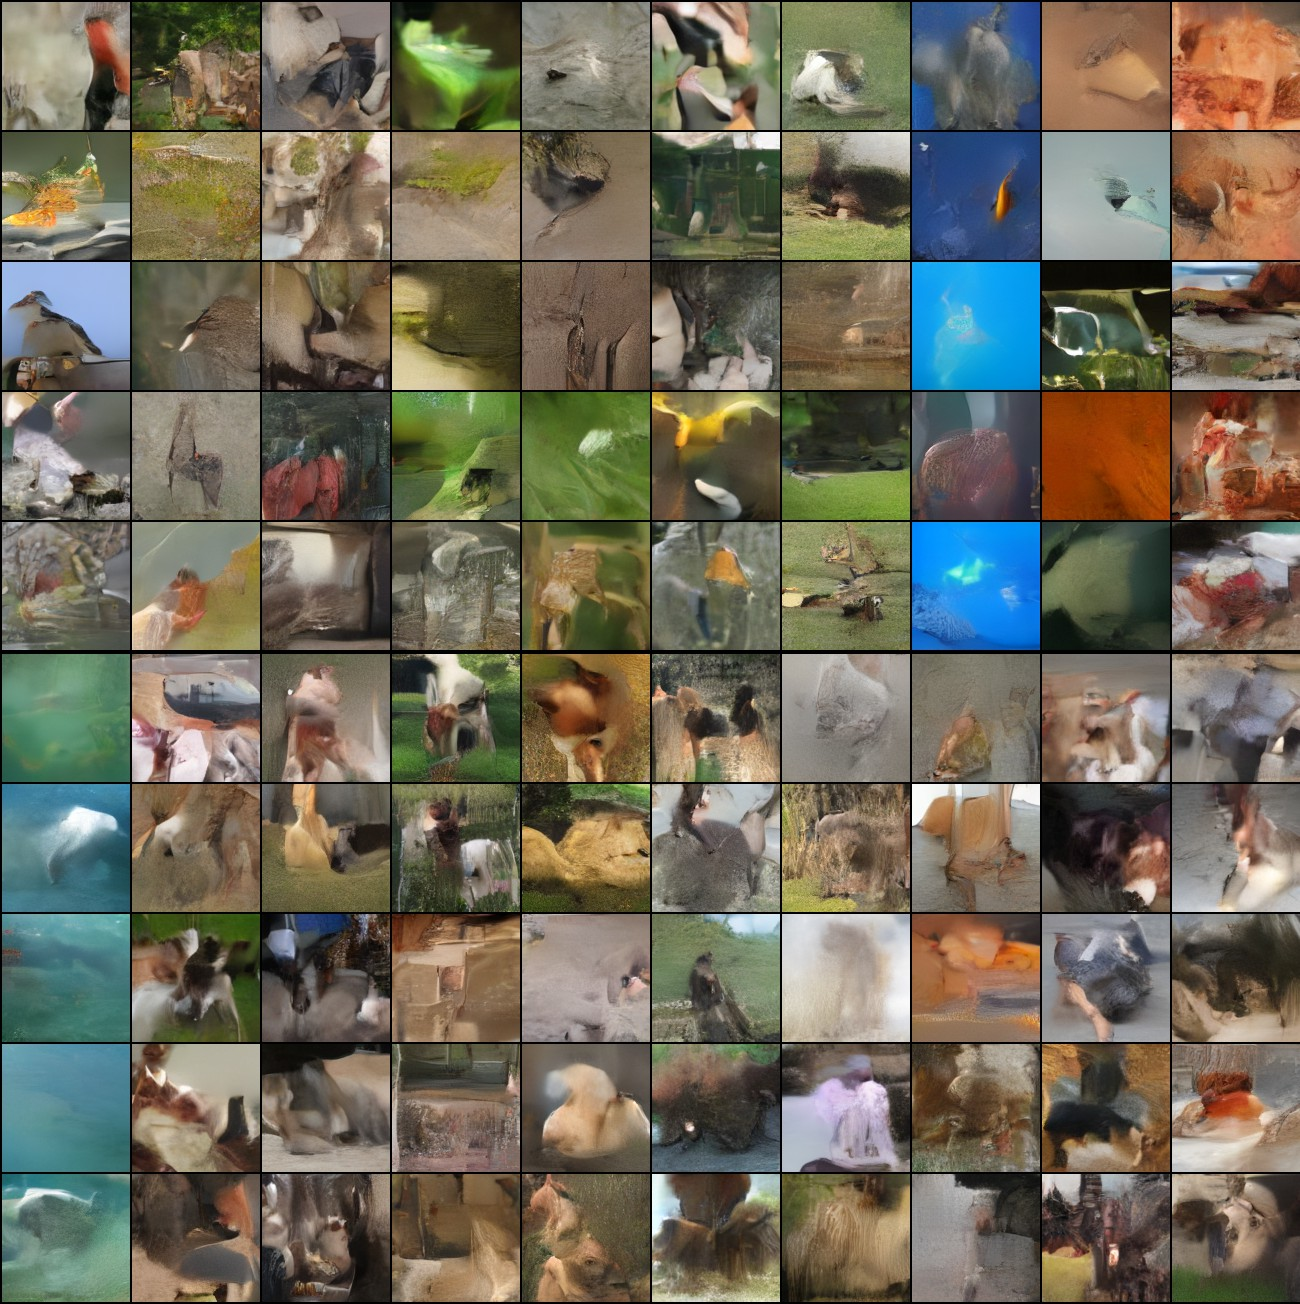
\includegraphics[width=\linewidth]{figs/mini_vit_ep39.jpg}\caption{epoch 40}\end{subfigure}
\begin{subfigure}{0.32\linewidth}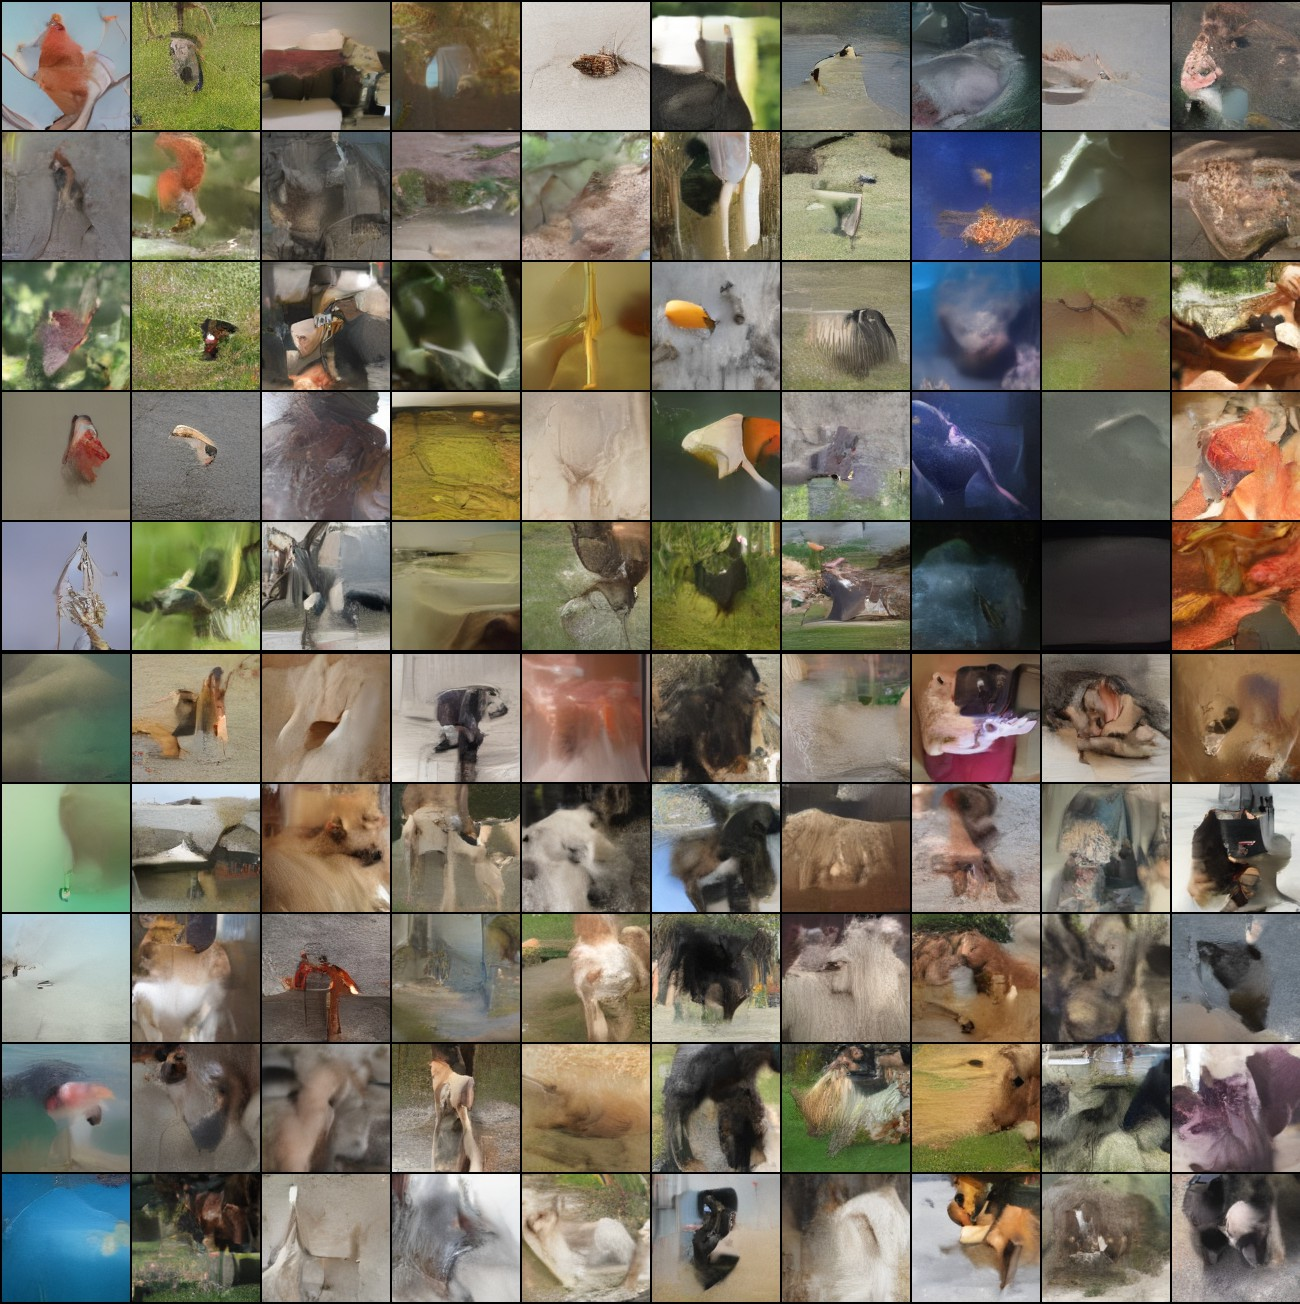
\includegraphics[width=\linewidth]{figs/mini_vit_ep79.jpg}\caption{epoch 80}\end{subfigure}
\caption{ViT samples during training (same classes as Fig.~\ref{fig:mini}).}
\label{fig:progress}
\end{figure}

\begin{table}[!htbp]
\centering
\begin{tabular}{lrrrrr}
\toprule
Backbone & Params & Final loss & Train time & s/iter & FID $\downarrow$ \\
\midrule
U-Net (dim 96) & 16.8M & 0.88 & 5h27m & 0.31 & 117.1 \\
ViT (depth 12, width 288) & 18.4M & 0.87 & 6h38m & 0.38 & \textbf{115.4} \\
\bottomrule
\end{tabular}
\caption{Latent FM on MiniImageNet (80 epochs, shared T4). FID from 5{,}000 generated images (50 per
class) against the test split, using the final EMA checkpoints. The ViT ran alone on the GPU for its
last hour, at 0.28 s/iter.}
\label{tab:mini}
\end{table}

\paragraph{Training curves.} Both losses drop quickly in the first few thousand iterations and then
decrease slowly with a lot of noise (Fig.~\ref{fig:curves}, right). The noise is normal for this kind of
training on varied natural images. The U-Net's loss falls faster at first, but the ViT overtakes it after
about 35{,}000 iterations and ends slightly lower (0.87 vs.\ 0.88).

\paragraph{Sample quality and FID.} The final FID scores are \textbf{117.1 for the U-Net and 115.4 for
the ViT}. These are far from state of the art, which is expected with 80 epochs, about 17M parameters,
10 sampling steps and no CFG. The samples have realistic colors, lighting, backgrounds and textures
(grass, water, fur, sky), and many are clearly related to their class. For example, column 8 shows blue
underwater scenes for both models, the ViT's first columns show small birds and orange-beaked birds, and
the bottom half produces furry, dog-like shapes. However, object shapes are usually distorted or
incomplete (for example, no clear dog faces), and some samples are blurry. Fig.~\ref{fig:progress} shows
how the samples improve: colored blobs at epoch 5, scene layouts with textured objects by epoch 40, and
gradual refinement afterwards.

\paragraph{Quality vs.\ computational cost.} The two backbones reach similar quality at similar size,
with the ViT slightly better in FID and final loss. On $16\times16$ latents with $2\times2$ patches the ViT
processes 64 tokens through 12 blocks. It was slower per iteration than the U-Net while both shared the
GPU (0.38 vs.\ 0.31\,s), so its small quality advantage came at a higher training cost (6h38m vs.\ 5h27m).
Sampling is cheap for both: 10 network calls plus one decoder call per image. Generating the 5{,}000 FID
images and computing FID took about 18 minutes for the ViT. A pixel-space model at $128\times128$ would
have needed a much larger network and far more GPU time.

\section{Bonus}
Not attempted.

\end{document}
